% !TEX root = mythesis.tex

%==============================================================================
\chapter{Introduction}
\label{sec:intro}
%==============================================================================
\begin{figure}[h!]
\centering
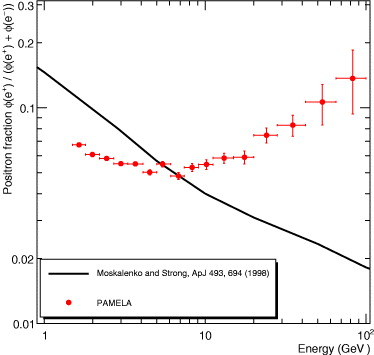
\includegraphics[width=9cm]{thesis_figures/nj317989fig13.jpg}
\caption{Positron fraction measured by PAMELA (red) along with a theoretical model (black)~\cite{Cholis_2009}}
\label{fig:PAMELA}
\end{figure}
Questions like \textit{How? Why? When?} have always been part of a scientist's vernacular and describe the fundamental need for humans in general to know the inner workings of every process we can observe or predict. A similar need that began as a philosophical thought of Democritus, the first person to use the term atom, was further refined by John Dalton in his "Atomic Model" and was turned into a real observable quantity for the first time by JJ. Thompson~\cite{SMITH1997}, setting up the foundations for one of the pioneer fields of science we call particle physics. Particle physics has led us very close to the ultimate goal which is to fully link and explain all aspects of the physical universe. It tries to describe every known phenomena as fundamentally as possible by reducing all known processes to an interaction between elementary particles governed by four known forces. The current theory which classifies all known elementary particles and incorporates three of the four known fundamental forces is called the Standard Model (SM)~\cite{Book_SM}. The current formulation of the theory which is accredited to a large collaborative effort was arrived upon in the late 1970s~\cite{GLASHOW1961579,PhysRevLett.19.1264,10025429448}. The SM classifies elementary particles in two broad categories: Fermions and Bosons. Fermions are the building blocks of matter and are further divided into quarks and leptons. Bosons which are the force carriers or messenger particles are divided into Gauge ($\gamma, W^{+/-} ,Z ,g$) and Scalar ($H$) bosons and mediate the strong($g$), weak ($W^{+/-}/Z$), and electromagnetic ($\gamma$) forces. The gravitational force is not included in the SM but a hypothetical mediator gauge boson graviton ($G$) has been suggested. Since it's publication the SM has been rigorously tested for it's several predictions with various experiments~\cite{RevModPhys.71.S96} and the decisive observation of Higgs boson by ATLAS~\cite{Aad_2012} and CMS~\cite{Chatrchyan_2012} in 2010 established it as a widely accepted theory.

\begin{figure}[t!]
\centering
  \begin{minipage}[t]{.45\textwidth}
    \centering
    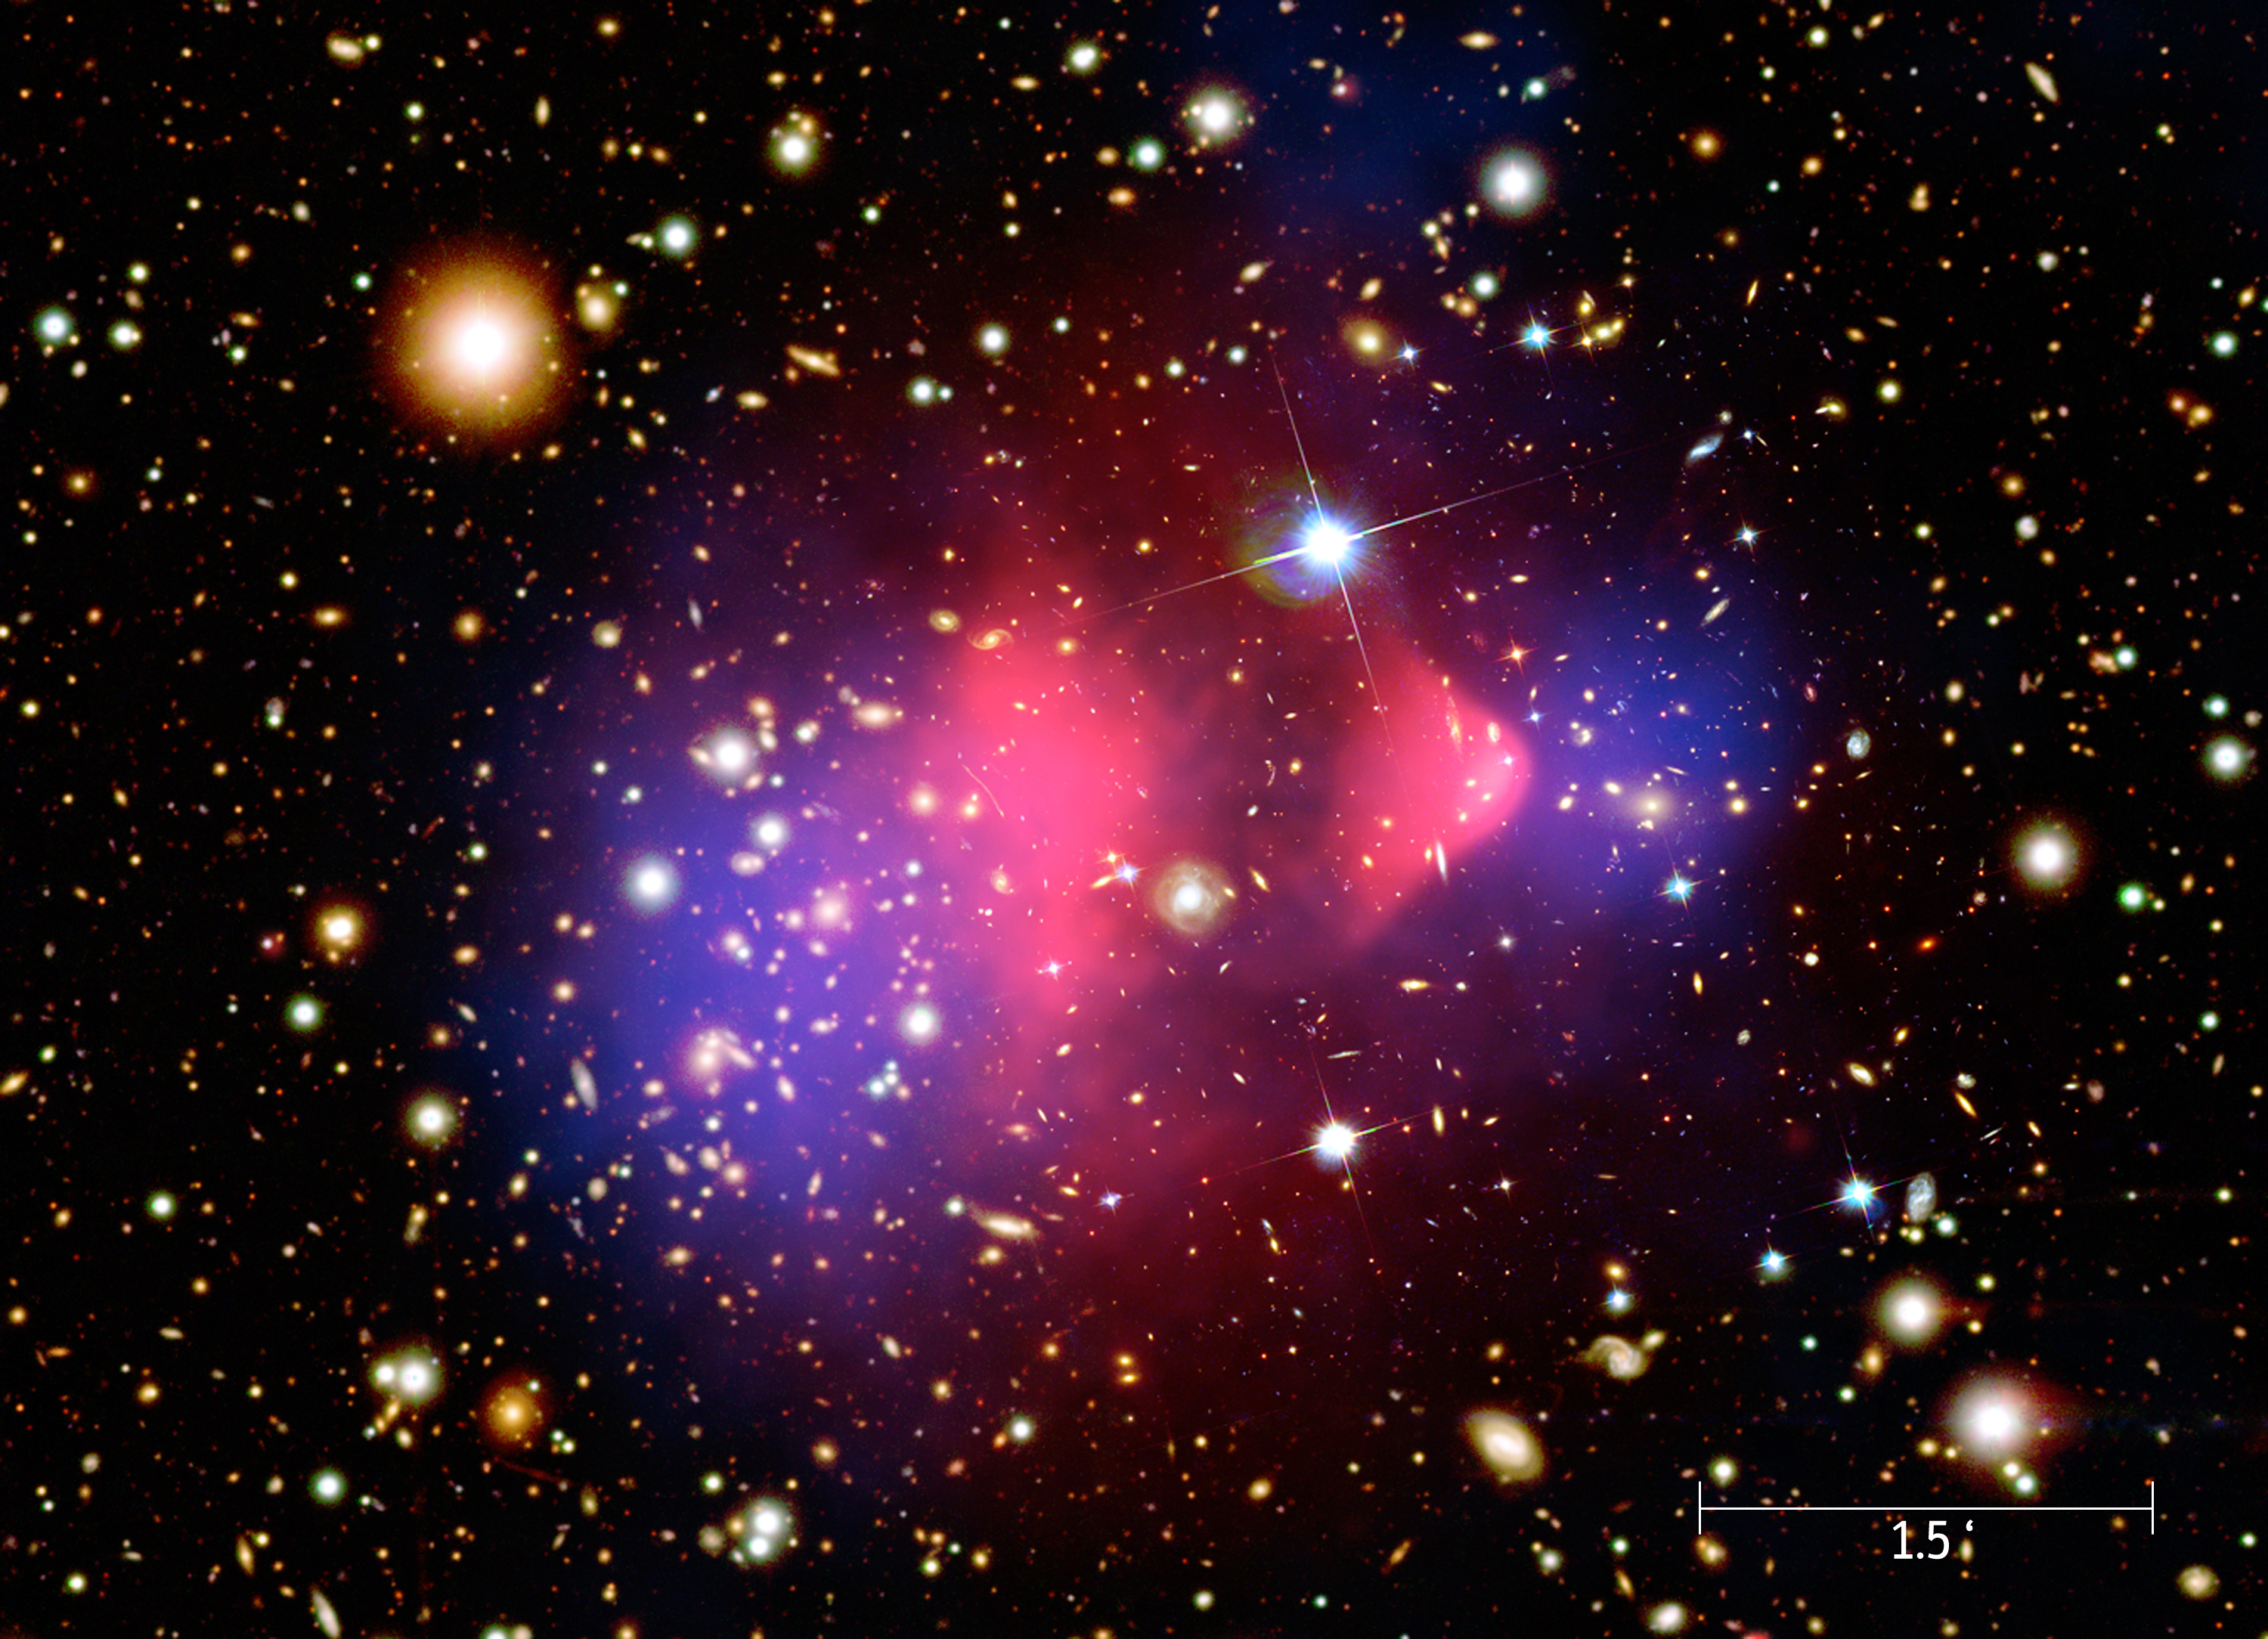
\includegraphics[width=\linewidth]{thesis_figures/bullet_cluster_final.jpg}

    \caption{Composite image of the bullet cluster. The x-ray emission recorded by Chandra telescope is shown in pink. The blue overlay is the mass distribution of the clusters calculated from gravitational lensing effects. ~\cite{NASA}.}
    \label{fig:Bullet2}
  \end{minipage}
  \hfill
  \begin{minipage}[t]{.45\textwidth}
    \centering
    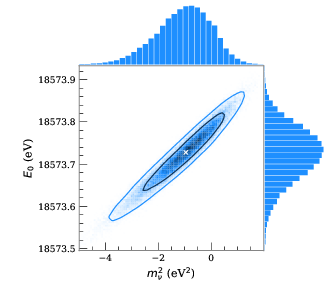
\includegraphics[width=\linewidth]{thesis_figures/neutrino_KATRIN.png}
    \caption{Scatter plot of fit values for the neutrino mass square and the effective $\beta$-decay endpoint E0 together with 1-$\sigma$ (black) and 2-$\sigma$ (blue) error contours around the best fit point (cross).~\cite{Aker:2019uuj}}
    \label{fig:neutrino_mass}
  \end{minipage}
\end{figure}
Although the SM describes most of the known processes, there are still several phenomena which remain unexplained leading us to look for modifications or alternate theories that can supplement the SM. The observations of PAMELA~\cite{Cholis_2009} which present a clear matter-antimatter asymmetry find no clear explanations in the SM. The discovery of neutrino oscillations~\cite{Fukuda_1998} which leads to a non-zero neutrino mass~\cite{Aker:2019uuj} is still not fully incorporated in the SM even with the proposed modifications~\cite{Mohapatra_2007}. Further challenges to the SM arrive from cosmological observations such as the accelerated expansion~\cite{RevModPhys.84.1151}, the discrepancies in the calculated mass of the Bullet cluster~\cite{Clowe_2004} and the Cosmic Microwave Background measurements (CMB) by WMAP/PLANCK~\cite{Bennett_2013,Aghanim:2018eyx}, which have led to a drastic change in our understanding of the composition of the known universe, one which consists of only 4.9\% ordinary matter, i.e the matter described by the SM. The other 95.1\%, distributed as 26.8\% dark matter and 68.3\% dark energy, finds no explanation in the SM. The theoretical developments or modifications needed to rectify the shortcomings of the SM are referred to as Physics Beyond the Standard Model (BSM).

To further expand our knowledge of the universe, especially the dark matter puzzle, numerous candidates have been proposed with their observations dependent on interactions with SM particles. Among them Weakly Interacting Massive Particles (WIMPs)~\cite{Jungman_1996} and axions~\cite{raffelt1995axions} are some of the more popular search prospects. Another candidate, which is the focus of this thesis, is the Dark Photon $A'$ also known as hidden, heavy, para-, or secluded photon. As the name suggests the Dark Photon is hypothesized to be a photon-like force carrier for dark matter. The theory and motivation behind $A'$ and its interaction with the SM will be discussed in more detail in chapter(\ref{sec:darkp}).

\begin{figure}[h!]
\centering
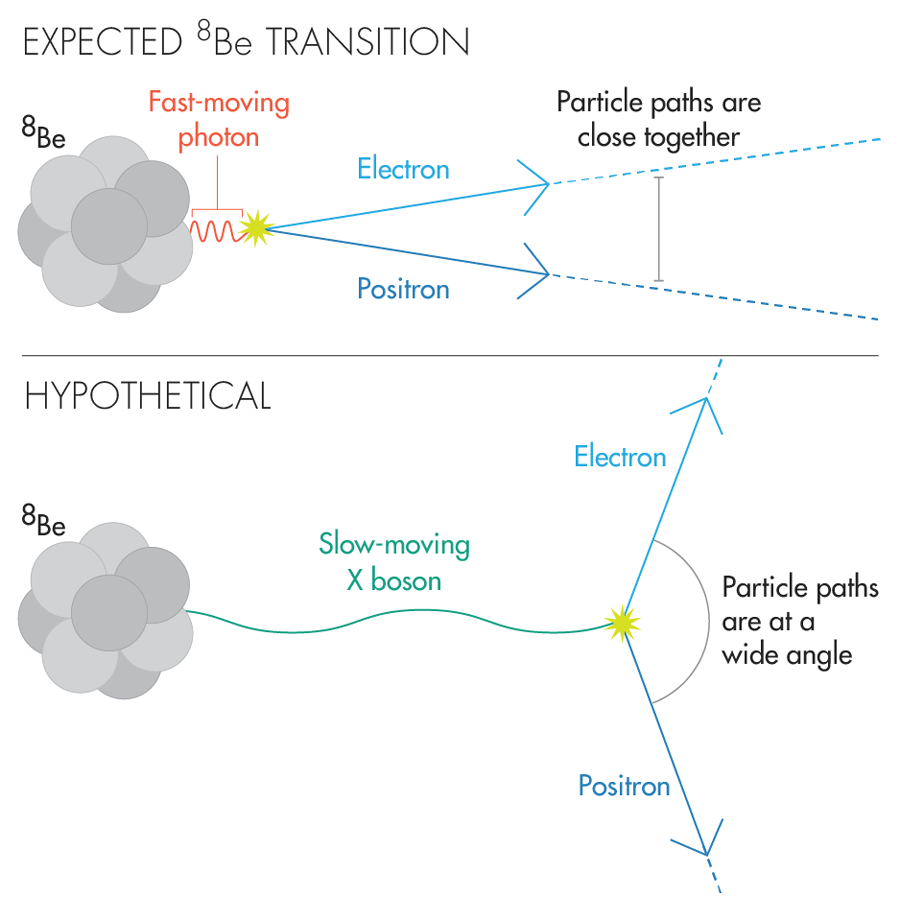
\includegraphics[width=8cm]{thesis_figures/VectorBoson_450.png}
\caption{Hypothesized X17 Boson production~\cite{Quanta_magazine}}
\label{fig:ATOMKI}
\end{figure}

The experiments which look for these speculated particles can be broadly divided into two categories "Direct" and "Indirect" detection, based on which part of the decay chain they are tuned to observe. Direct detection experiments try to measure the low-energy recoil of atomic nuclei when they are hit by Dark Matter (DM) particles passing through the Earth. Some examples of these laboratories which are usually situated miles underground to observe these rare processes are Xenon1T~\cite{PhysRevLett.121.111302} and LUX~\cite{Akerib_2017}, both of which are looking for WIMPs. On the other hand Indirect detection experiments try to look for products of decay or annihilation of dark matter particles. In this sector the scale of viable areas to look for is literally astronomical. The signature of such events can be in myriad forms such as neutrinos, high-energy gamma rays or even cosmic rays to name a few. Some experiments looking for corresponding signals are IceCube, ANTARES (both neutrinos)~\cite{IceCube2018MultimessengerOO,Adri_n_Mart_nez_2016}, Fermi Gamma-ray Space Telescope (gamma-rays)~\cite{Hooper_2011} and  Alpha Magnetic Spectrometer (cosmic-rays)~\cite{PhysRevLett.118.191101}.
Indirect searches also involve accelerator experiments~\cite{essig2013dark} where dark matter particles can be produced and detected as either missing energy (invisible) or an excess of final products (visible). One of such experiments looking for the Dark Photon $A'$ in a beam dump experiment is NA64~\cite{andreas2013proposal}, which has been consistently trying to estimate the theorized properties of $A'$. It has also played a role in constraining the coupling and mass of DM particle $\chi$ and the hypothesized 16.7 MeV boson (X17) first observed by the ATOMKI experiment~\cite{Krasznahorkay_2016,krasznahorkay2019new}.

This thesis presents the work done to implement a data analysis chain for the NA64 experiment in COmpass Reconstruction AnaLysis software package(CORAL)~\cite{Collaboration2007TheCE}. The work involves setting up an alignment chain for different experimental setups of NA64 incorporating the inbuilt Millepede minimization tool of CORAL. The alignment is further verified by comparing it to the standalone tool described in~\cite{nabeel:2018}. It further involves studying and documenting the already implemented Monte Carlo (MC) simulation for NA64 and translating the output to a format compatible with CORAL for reconstruction. Finally the obtained CORAL MC reconstruction is checked with the published studies~\cite{PhysRevD.97.072002}.
%%% Local Variables:
%%% mode: latex
%%% TeX-master: "mythesis"
%%% End:
